\chapter{Lebenslauf}\vspace{1cm}
\begin{vwcol}[widths={0.4,0.6}, rule=0.4pt, sep=.5em, indent=.5em]
%linke Seite:
  \begin{centering}
  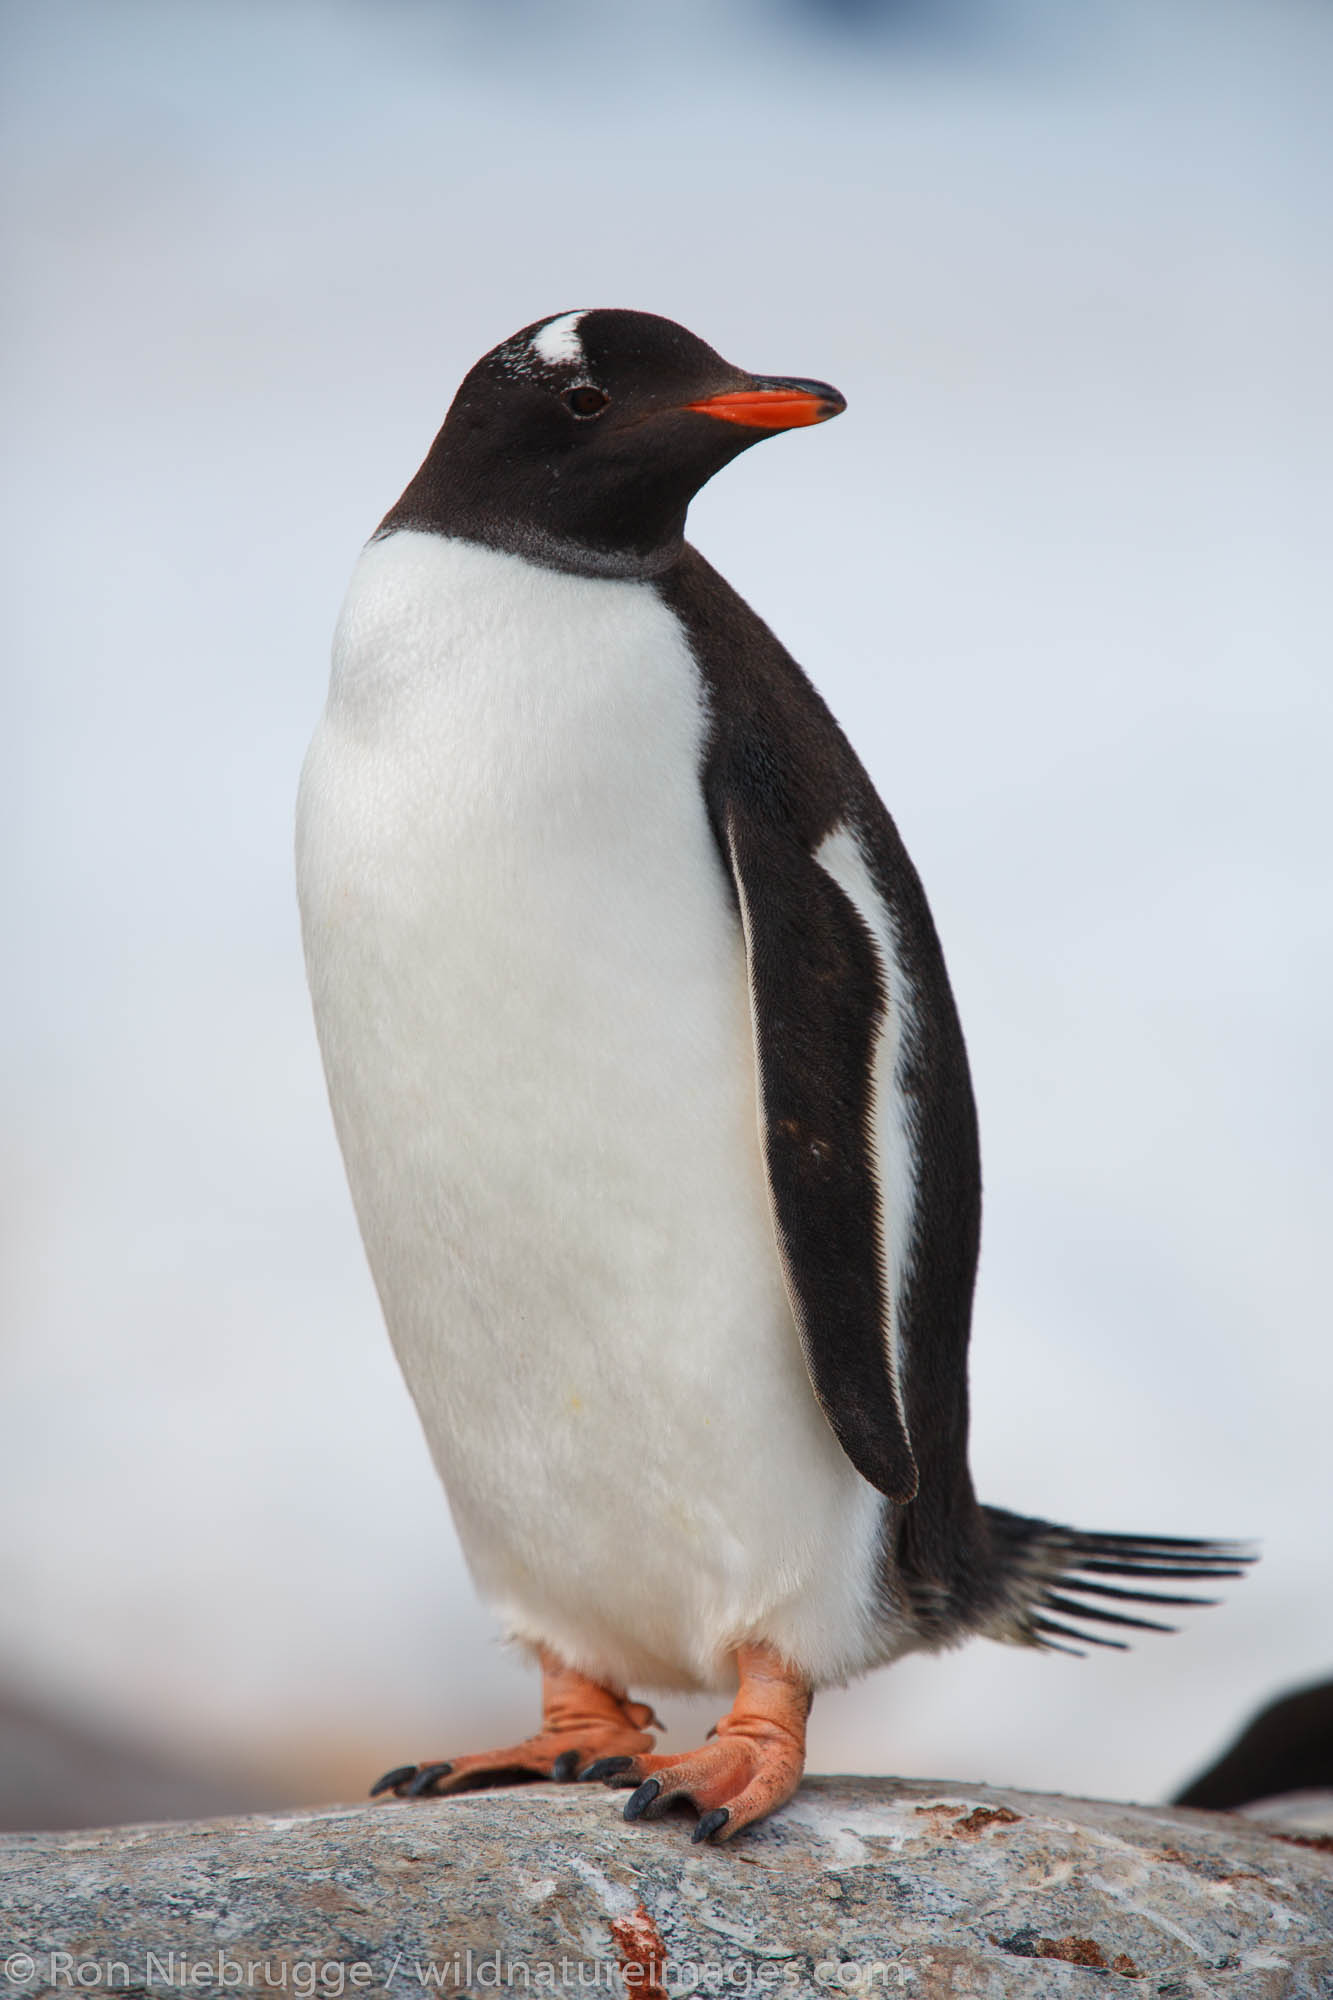
\includegraphics[width=4cm]{./Profile_Pic.jpg}\\
%TODO: Feel free to change the information for your needs.
  \Large\textbf{Kontaktdaten}\\
  \normalsize
  Max Mustermann\\
  Adresse: Musterstraße X, PLZ Musterstadt\\
  Geburtsdatum: XX.XX.XXXX\\
  Geburtsort: Musterort\\
  Mail: \href{mailto:muster@muster.de}{muster@muster.de}\\
  Telefon: \href{tel:+XXXXXXXXXX}{+XX XXX XXXXXXX}\\
  Links: \LARGE \hspace{0.2 cm} \href{https://www.linkedin.com/muster}{\faLinkedin} \hspace{0.5 cm}\href{https://github.com/muster}{\faGithub} \hspace{0.5 cm}\href{https://www.instagram.com/muster/}{\faInstagram}\\\vspace{0.8cm}

  \Large\textbf{Kenntnisse}\\
  \end{centering}  \normalsize
  \hyperref[<reference>]{Sprachen}\\
  L\href{<reference_url>}{atex}\\

  \vspace{0.8cm}

  \begin{centering}
    \Large\textbf{Interessen}\\
  \end{centering}\normalsize
 Sport\\
  Musik\\
  \pagebreak


%rechte Seite:
  \Large\textbf{Ausbildung}\\
  \normalsize
  \begin{tabular}{rl}
  & \\
  20XX - 20XX & \textbf{Bachelor}\\
  & Universität X\\
  & \textit{\hyperref[Bachelorzeugnis]{Abschlussnote: 4,0}}\\
  
  20XX - 20XX & \textbf{Allgemeine Hochschulreife}\\
  & Gymnasium X\\
  & \textit{\hyperref[Abiturzeugnis]{Abschlussnote: 4,0}}\\
  \end{tabular}\\\vspace{0.8cm}

  \Large\textbf{Erfahrung}\\
  \normalsize
  \begin{tabular}{ll}
  & \\
  20XX - 20XX & \textbf{Eherenamtliche Arbeit}\\
    & Verein X \\
    & \textit{Das hab ich da gemacht}\\
  20XX  & \textbf{Berufserfahrung}\\
    & Unternehmen X\\
    & \textit{Aufgabenfeld}\\
  \end{tabular}\\\vspace{0.8cm}

  \Large\textbf{Referenzen}\\\normalsize
  \begin{tabular}{l}
    \\
    Prof. Dr. phil. habil. Musterprof\\
    Mail: \href{mailto:muster@muster.de}{muster@muster.de}\\
    Telefon: \href{tel:+XXXXXXX}{+XX XXX XXXXXXXX}
  \end{tabular}
\end{vwcol}